\documentclass{article}
\usepackage{amsmath}
\usepackage[utf8]{inputenc}
\usepackage{natbib}
\usepackage{graphicx}
\usepackage{caption}
\usepackage{subcaption}

\title{LELEC2103:Labview5}
\author{Bronchain Olivier \\ Schellekens Vincent}
\date{\today}

\begin{document}
\maketitle
\section{Pre-lab}
	\subsection{Error on the estimate delay in the channel}
		Let observe what append if we get a estimated delay wrongly estimated. Due to noise the maximum value of the correlation can be shifted of more than a symbol period. This cause a wrong delay estimation. The signal will be shifted of a wrong delay and will cause a BER near to 0,5. Let see this little example. \\ 
		\begin{figure}[h!]
			\centering
			\begin{tabular}{|c|| c | c | c | c | c | c | c | c |}
				\hline
				Sample & 1 & 2 & 3 & 4 & 5 & 6 & 7 & 8 \\ 
				\hline
				\hline 
				Excepted recieved signal (training sequence) & 10 & 11 & 10 & 00 & 10 & 11 & 10 & 00 \\
				\hline
				Received sequence & 10 & 00 & 10 & 11 & 10 & 00  & XX & XX \\
				\hline
			\end{tabular}
			\caption{Recieved sequence vs excpeted sequence with a $d=2$ \label{f1}}	
		\end{figure}
	
		Due to noise we won't get $\hat{d}=2$ as expected but $\hat{d}=1$. The corrected recieved sequence is then shifted of $\hat{d}=1$ (Figure \ref{f2}). \\ 
		\begin{figure}[h!]
			\centering
			\begin{tabular}{|c||c|c|c|c|c|c|c|c|}
				\hline
				Sample & 1 & 2 & 3 & 4 & 5 & 6 & 7 & 8 \\
				\hline
				\hline 
				Excepted recieved signal (training sequence) & 10 & 11 & 10 & 00 & 10 & 11 & 10 & 00 \\
				\hline
				Corrected sequence & 11 & 10 & 00 & 10 & 11 & 10 & 00 & XX \\
				\hline		
			\end{tabular}
			\caption{Corrected sequence vs expected sequence with a $\hat{d}=1$ \label{f2}}
		\end{figure}
		We see on Figure \ref{f2} that sequence is badly corrected. A symbol is not at the same place in the sequence then it should be. It will cause a $BER \simeq 0.5$. 
	\subsection{Influence of frequency offset}
		The recieved signal is given by Equation \ref{rec}.
		\begin{equation}
			y[h] = e^{j2\pi nT\Delta f} \sum _{l=0}^{L} h[l]s[n-l]+v[n]
			\label{rec}
		\end{equation}
		Where $\Delta f$ is the frequency offset between the transmitter and the receiver. The effect of it is that the symbols are shifted of a phase propotinal to there position in the received sequence and to the $\Delta f$.
		 \begin{figure}[h!]
	            \centering  
	            \begin{subfigure}[b]{0.3 \textwidth}
	                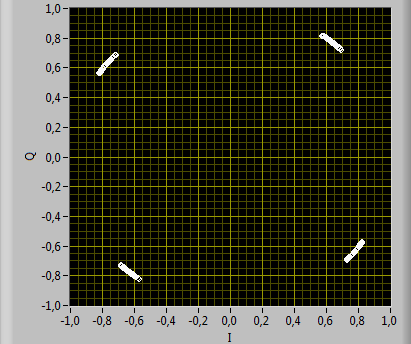
\includegraphics[width=\textwidth]{off100.PNG}
	                \caption{$\Delta f = 100Hz$}\label{fig:2}
	            \end{subfigure}
	            ~	           
	            \begin{subfigure}[b]{0.3 \textwidth}
	           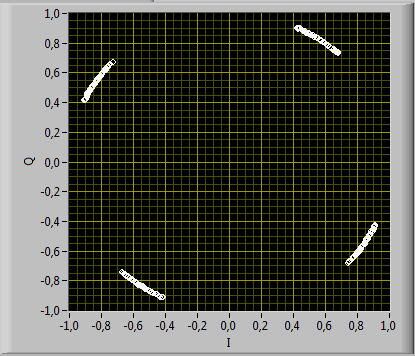
\includegraphics[width=\textwidth]{off201.PNG}
	                \caption{$\Delta f = 201Hz$}\label{fig:4}
	            \end{subfigure}
	            
	            \begin{subfigure}[b]{0.3 \textwidth}
	                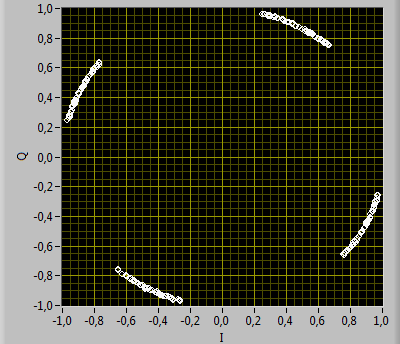
\includegraphics[width=\textwidth]{off300.PNG}
	                \caption{$\Delta f = 300Hz$}\label{fig:10}
	            \end{subfigure}
	            ~	           
	            \begin{subfigure}[b]{0.3 \textwidth}
	           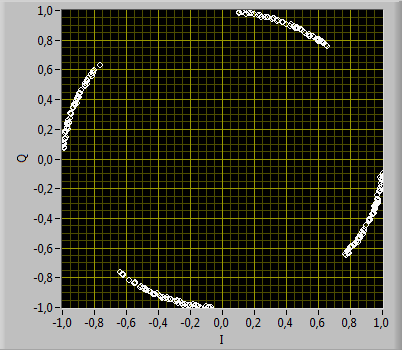
\includegraphics[width=\textwidth]{off400.PNG}
	                \caption{$\Delta f = 400Hz$}\label{fig:20}
	            \end{subfigure}
	            \caption{Received constellation with a frequency offset}\label{fig:shi}
	        \end{figure}	

		Due to periodicity of the phase there is some limiation to the system. 
		$$ 2\pi N_t T \Delta f < \frac{ \pi}{2}$$
		$$ \Delta f < \frac{1}{4 N_t T}$$
			
\section{Lab}
	\subsection{Frequency offset correction}
		We observe the frequency correction on a real wireless link. The native frequency offset was estimated around $5Hz$. We introduce a artificial offset in the system and observe the frequency correction works well if we don't goes off the maximal frequency ( estimated to $2,2Hz$ with the parameters of the system)(see Figure \ref{BER}).
		\begin{figure}[h!]
			\centering
			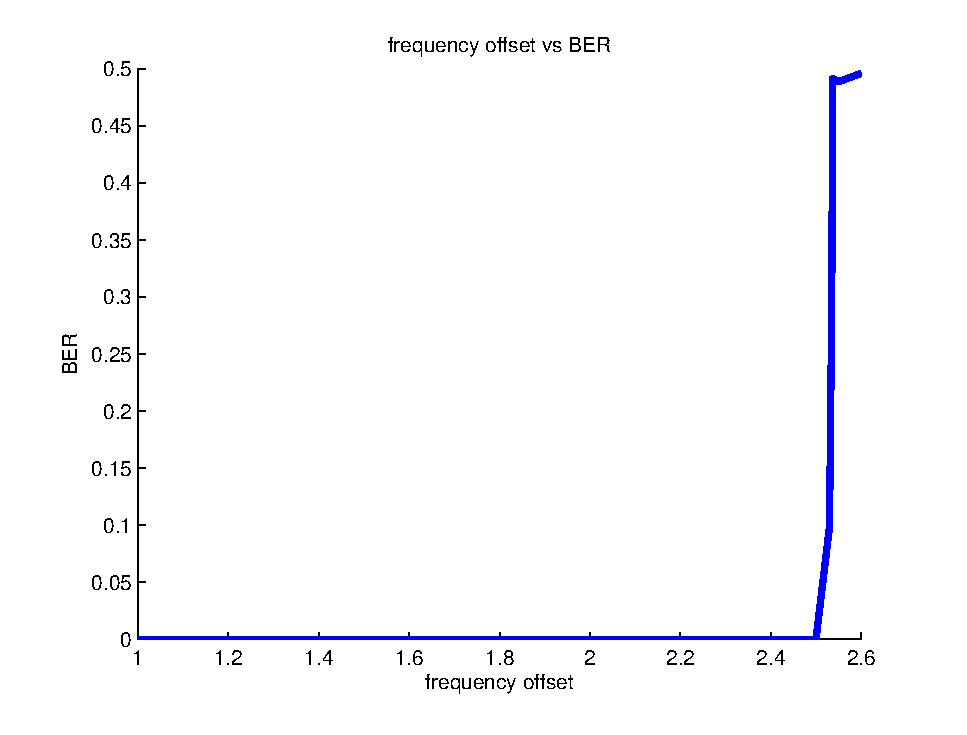
\includegraphics[width = 0.5 \textwidth]{ber.eps}
			\caption{Frequency offset vs BER \label{BER}}
		\end{figure}	
	\subsection{Self referenced frame synchronization}


\end{document}
